\documentclass[12pt,a4paper]{article}
\usepackage[utf8]{inputenc}
\usepackage[margin=1in]{geometry}
\usepackage{amsmath}
\usepackage{amsfonts}
\usepackage{amssymb}
\usepackage{graphicx}
\usepackage{listings}
\usepackage{xcolor}
\usepackage{fancyhdr}
\usepackage{titlesec}
\usepackage{tikz}
\usepackage{enumerate}
\usetikzlibrary{positioning,shapes,arrows}
\usepackage[colorlinks=true, linkcolor=blue, urlcolor=blue, citecolor=blue]{hyperref}
\usepackage{tcolorbox}

% Define question box style
\newtcolorbox{questionbox}{
    colback=blue!5!white,
    colframe=blue!75!black,
    fonttitle=\bfseries,
    title=Question,
    sharp corners,
    boxrule=1pt,
    left=8pt,
    right=8pt,
    top=8pt,
    bottom=8pt
}

% SQL syntax highlighting
\lstdefinestyle{sqlstyle}{
    language=SQL,
    basicstyle=\ttfamily\small,
    keywordstyle=\color{blue}\bfseries,
    commentstyle=\color{green!50!black},
    stringstyle=\color{red},
    numbers=left,
    numberstyle=\tiny\color{gray},
    numbersep=5pt,
    breaklines=true,
    breakatwhitespace=true,
    tabsize=2,
    showspaces=false,
    showstringspaces=false,
    frame=single,
    rulecolor=\color{gray!30},
    backgroundcolor=\color{gray!5}
}

\lstset{style=sqlstyle}

% Page setup
\pagestyle{fancy}
\fancyhf{}
\rhead{CSE 414 - Assignment 7}
\lhead{Database Systems}
\cfoot{\thepage}

% Title formatting
\titleformat{\section}{\Large\bfseries}{}{0em}{}
\titleformat{\subsection}{\large\bfseries}{}{0em}{}

\begin{document}

% Title Page
\begin{titlepage}
    \begin{figure}[htbp]
    \centering
    
\includegraphics[width=0.2\textwidth]{cu.png}
    \end{figure}
    \centering
    \vspace*{0.5cm}
    {\Huge\bfseries University of Chittagong}\\[0.5cm]
    {\Large Department of Computer Science \& Engineering}\\[0.5cm]
    {\large Database Systems Lab}\\[2cm]
    
    {\large Name of the assignment:}\\[0.3cm]
    {\LARGE\bfseries Assignment 7: Chapter 7 Exercise\\[0.5cm]}
    {\large CSE 414}\\[0.5cm]
    {\large Database Systems}\\[3.5cm]
    
    \begin{minipage}[t]{0.4\textwidth}
    \raggedleft
    Submitted By:\\
    \large \textbf{Debashish Chakraborty}\\
    \large ID: 23701034
    \end{minipage}              
    \hspace{0.05\textwidth}
    \vrule width 1pt
    \hspace{0.05\textwidth}
    \begin{minipage}[t]{0.4\textwidth}
    Submitted To:\\
    \large \textbf{Dr. Rudra Pratap Deb Nath}\\
    \large Associate Professor
    \end{minipage}
    
    \vfill
    {\large July 7, 2025}
\end{titlepage}

\newpage

\section{Problem 7.8: Algorithm Efficiency Analysis}

\begin{questionbox}
\textbf{7.8:} Consider the algorithm in Figure 7.19 to compute $\alpha^+$. Show that this algorithm is more efficient than the one presented in Figure 7.8 (Section 7.4.2) and that it computes $\alpha^+$ correctly.
\end{questionbox}
\newline


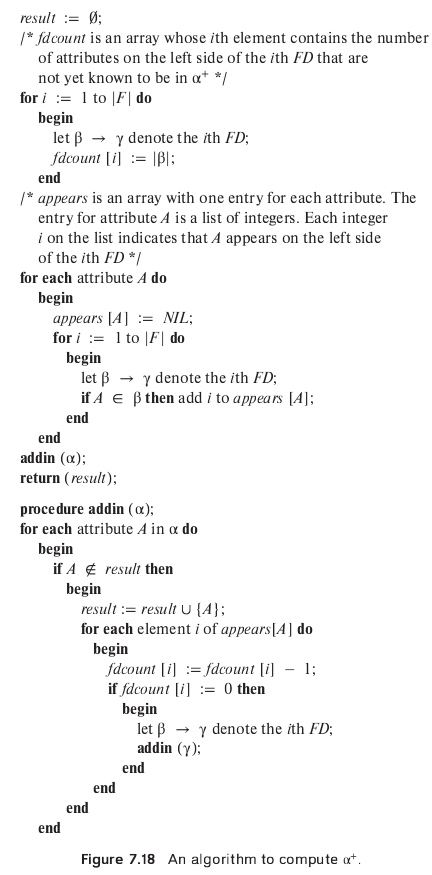
\includegraphics[width=0.6\textwidth]{Figure7.18.png}
\newpage

\textbf{Solution:}

The given algorithm's goal is to compute $\alpha^+$.

\begin{enumerate}
    \item Initially, all attributes in $\alpha$ are added to the result.
    \item For each FD $\beta \rightarrow \gamma$, the algorithm tracks how many attributes from $\beta$ are still missing using an array \texttt{fdcount}.
    \item \texttt{appears[A]} lists all FDs where attribute $A$ appears in the LHS.
    \item When an attribute $A$ is added to the result, the algorithm checks all FDs waiting for $A$ via \texttt{appears[A]}.
    \item If all attributes in the LHS $\beta$ of some FD are now in the result (\texttt{fdcount[i]} becomes 0), the corresponding RHS $\gamma$ is recursively added to the result.
\end{enumerate}\\
\\
\textcolor{blue}{\textbf{Why is it correct?}}\\
Every attribute $A$ added to the result has a valid derivation $\alpha \rightarrow A$ based on FDs. This is ensured because $A$ is only added when there is a dependency $\beta \rightarrow \gamma$ such that $\beta \subseteq \alpha^+$ and $A \in \gamma$.
    
 If $A \in \alpha^+$, then $A$ will be added to the result. This is provable by induction on the length of the proof of $\alpha \rightarrow A$ using Armstrong's axioms:
    \begin{itemize}
        \item \textbf{Base Case:} If $A \in \alpha$, it is added in the initial call to \texttt{addin}.
        \item \textbf{Inductive Step:} Suppose $\alpha \rightarrow A$ is proven in $n+1$ steps. Then there must be some dependency $\beta \rightarrow \gamma$ with $\beta \subseteq \alpha^+$ and $A \in \gamma$. By inductive hypothesis, all of $\beta$ has already been added to the result, triggering the addition of $\gamma$, and thus $A$.
    \end{itemize}


\subsection*{Efficiency Analysis}

Let us now compare the performance of the two algorithms.\\

In \textbf{Figure 7.19}, each FD is scanned exactly once in the initialization phase to compute \texttt{fdcount} and \texttt{appears}. The recursive calls to \texttt{addin} process attributes only once and process only relevant FDs using \texttt{appears[A]}. So every FD and attribute is processed only when needed.\\

 In contrast, the algorithm in \textbf{Figure 7.8} repeatedly scans the entire FD set in a loop until no new attributes are added to the closure. In the worst case, this could result in $O(|F|^2)$ time complexity if each FD triggers a new iteration.


\subsubsection*{Complexity Comparison}

{Algorithm in Figure 7.19:} $O(|F| + |R|)$ (linear in the size of FDs and attributes) \\
{Algorithm in Figure 7.8:} $O(|F|^2)$ (may scan all FDs multiple times)


\newpage
\section{Problem 7.26: Functional Dependency Rule Soundness}

\begin{questionbox}
\textbf{7.26:} Consider the following proposed rule for functional dependencies: If $\alpha \rightarrow \beta$ and $\gamma \rightarrow \beta$, then $\alpha \rightarrow \gamma$. Prove that this rule is not sound by showing a relation $r$ that satisfies $\alpha \rightarrow \beta$ and $\gamma \rightarrow \beta$, but does not satisfy $\alpha \rightarrow \gamma$.
\end{questionbox}

\textbf{Solution:}

We can prove that this rule is not sound by providing an example. Consider the following relation $R$:

\begin{center}
\begin{tabular}{|c|c|c|}
\hline
$\alpha$ & $\gamma$ & $\beta$ \\
\hline
A & X & 100 \\
B & Y & 200 \\
B & Z & 200 \\
\hline
\end{tabular}
\end{center}

In this relation:
\begin{itemize}
    \item $\alpha \rightarrow \beta$ holds: Each value of $\alpha$ maps to a unique value of $\beta$
    \begin{itemize}
        \item $\alpha = A$ maps to $\beta = 100$
        \item $\alpha = B$ maps to $\beta = 200$
    \end{itemize}
    
    \item $\gamma \rightarrow \beta$ holds: Each value of $\gamma$ maps to a unique value of $\beta$
    \begin{itemize}
        \item $\gamma = X$ maps to $\beta = 100$
        \item $\gamma = Y$ maps to $\beta = 200$
        \item $\gamma = Z$ maps to $\beta = 200$
    \end{itemize}
    
    \item However, $\alpha \rightarrow \gamma$ does \textbf{not} hold: The value $\alpha = B$ maps to two different values of $\gamma$ (both Y and Z)
\end{itemize}
Therefore, If $\alpha \rightarrow \beta$ and $\gamma \rightarrow \beta$, then $\alpha \rightarrow \gamma$, is not sound.
\newpage
\section{Problem 7.35: BCNF Decomposition and Lossless Property}

\begin{questionbox}
\textbf{7.35:} Although the BCNF algorithm ensures that the resulting decomposition is lossless, it is possible to have a schema and a decomposition that was not generated by the algorithm, that is in BCNF, and is not lossless. Give an example of such a schema and its decomposition.
\end{questionbox}


\textbf{Solution:}

Consider the schema $R = (A, B, C, D)$ with the following set $F$ of functional dependencies:

$F := \{AB \rightarrow C, CD \rightarrow A\}$

Consider the following decomposition of $R$:
\begin{align}
R_1 &= (A, B, C) \\
R_2 &= (A, C, D)
\end{align}

\subsection{BCNF Verification}

\textbf{For $R_1 = (A, B, C)$:}

Functional dependencies projected onto $R_1$:
$F_1 = \{AB \rightarrow C\}$

We need to check if $AB$ is a superkey for $R_1$:
$(AB)^+ = \{A, B, C\} \text{ (within } R_1 \text{)}$

Since $AB$ determines all attributes in $R_1$, it is a superkey. Therefore, $R_1$ is in BCNF.\\
\textbf{For $R_2 = (A, C, D)$:}

Functional dependencies projected onto $R_2$:
$F_2 = \{CD \rightarrow A\}$

We need to check if $CD$ is a superkey for $R_2$:
$(CD)^+ = \{A, C, D\} \text{ (within } R_2 \text{)}$

Since $CD$ determines all attributes in $R_2$, it is a superkey. Therefore, $R_2$ is in BCNF.

\subsection{Lossless Property Verification}

To check if the decomposition is lossless, we use the condition:
$(R_1 \cap R_2) \rightarrow R_1 \text{ or } (R_1 \cap R_2) \rightarrow R_2$

We have:
$R_1 \cap R_2 = \{A, B, C\} \cap \{A, C, D\} = \{A, C\}$

For lossless join, we need either:
\begin{enumerate}
    \item $AC \rightarrow ABC$ (which means $AC \rightarrow B$), or
    \item $AC \rightarrow ACD$ (which means $AC \rightarrow D$)
\end{enumerate}

From the given FDs $\{AB \rightarrow C, CD \rightarrow A\}$, we cannot derive $AC \rightarrow B$.
$AC$ does not determine $B$.

From the given FDs $\{AB \rightarrow C, CD \rightarrow A\}$, we cannot derive $AC \rightarrow D$.
$AC$ does not determine $D$.

Since neither condition holds, the decomposition is \textbf{lossy}.


This example demonstrates that it is possible to have a BCNF decomposition that is not lossless.

\end{document}